% Generated by analysis/make_tikz_figures.py. Edit the script, not this file.
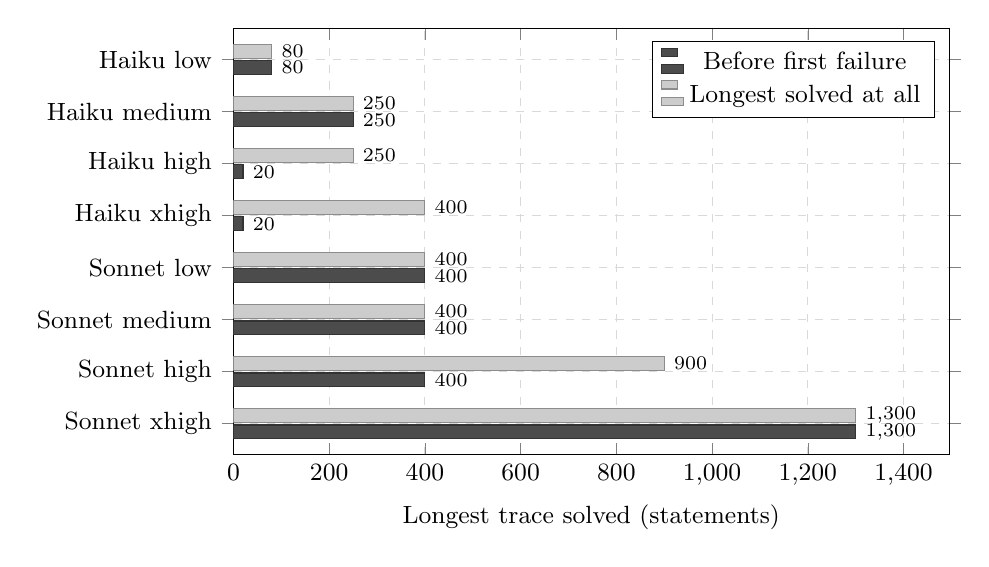
\begin{tikzpicture}
\begin{axis}[
  width=0.88\linewidth,
  height=7cm,
  grid=major,
  grid style={dashed, gray!30},
  tick label style={font=\small},
  label style={font=\small},
  xbar,
  bar width=5pt,
  xmin=0,
  xmax=1495,
  xtick distance=200,
  xlabel={Longest trace solved (statements)},
  ytick={8,7,6,5,4,3,2,1},
  yticklabels={Haiku low,Haiku medium,Haiku high,Haiku xhigh,Sonnet low,Sonnet medium,Sonnet high,Sonnet xhigh},
  ymin=0.4,
  ymax=8.6,
  nodes near coords,
  every node near coord/.append style={font=\scriptsize},
  legend style={at={(0.98,0.97)}, anchor=north east, font=\small},
]
\addplot[fill=black!70, draw=black!80, bar shift=-3pt] coordinates {(80,8) (250,7) (20,6) (20,5) (400,4) (400,3) (400,2) (1300,1)};
\addlegendentry{Before first failure}
\addplot[fill=black!20, draw=black!45, bar shift=3pt] coordinates {(80,8) (250,7) (250,6) (400,5) (400,4) (400,3) (900,2) (1300,1)};
\addlegendentry{Longest solved at all}
\end{axis}
\end{tikzpicture}
